% !TEX program = xelatex
\documentclass[UTF8,12pt,a4paper]{ctexart}

\usepackage[a4paper,top=2.5cm,bottom=2.5cm,left=2.7cm,right=2.7cm]{geometry}
\usepackage{amsmath,amssymb}
\usepackage{booktabs}
\usepackage{tabularx}
\usepackage{multirow}
\usepackage{graphicx}
\usepackage{float}
\usepackage[section]{placeins}
\usepackage{caption}
\usepackage{xcolor}
\usepackage{enumitem}
\usepackage{microtype}
\usepackage{cite}
\usepackage{hyperref}
\graphicspath{{figures/}}

\definecolor{linkblue}{RGB}{39,87,132}
\definecolor{softblue}{RGB}{232,241,248}
\definecolor{softgray}{RGB}{245,246,247}
\hypersetup{
  hidelinks,
  pdfauthor={},
  pdftitle={面向固定长度数字验证码的位置保持轻量级卷积网络设计与实验分析}
}

\setlength{\parindent}{2em}
\setlength{\parskip}{0pt}
\linespread{1.28}
\setlength{\emergencystretch}{2em}
\captionsetup{font=small,labelsep=quad}
\setlist[itemize]{leftmargin=2.2em,itemsep=0.15em,topsep=0.25em}
\setlist[enumerate]{leftmargin=2.2em,itemsep=0.15em,topsep=0.25em}

% 采用普通研究论文版式：无独立封面、无作者/学号/课程/学院栏。
\ctexset{
  section = {
    format = \zihao{3}\heiti,
    beforeskip = 1.4ex plus 0.4ex minus 0.2ex,
    afterskip = 0.8ex plus 0.2ex
  },
  subsection = {
    format = \zihao{4}\heiti,
    beforeskip = 1.1ex plus 0.3ex minus 0.2ex,
    afterskip = 0.5ex plus 0.2ex
  }
}
\pagestyle{plain}

\begin{document}
% 在首次编译、aux 尚无引用编号时提供固定编号；后续编译会直接使用 aux 中的编号。
% 编号与文末 thebibliography 的条目顺序保持一致。
\makeatletter
\@ifundefined{b@vonahn2003captcha}{\expandafter\gdef\csname b@vonahn2003captcha\endcsname{1}}{}
\@ifundefined{b@chen2017survey}{\expandafter\gdef\csname b@chen2017survey\endcsname{2}}{}
\@ifundefined{b@goodfellow2014multidigit}{\expandafter\gdef\csname b@goodfellow2014multidigit\endcsname{3}}{}
\@ifundefined{b@graves2006ctc}{\expandafter\gdef\csname b@graves2006ctc\endcsname{4}}{}
\@ifundefined{b@shi2017crnn}{\expandafter\gdef\csname b@shi2017crnn\endcsname{5}}{}
\@ifundefined{b@thobhani2020captcha}{\expandafter\gdef\csname b@thobhani2020captcha\endcsname{6}}{}
\@ifundefined{b@ma2020neuralcaptcha}{\expandafter\gdef\csname b@ma2020neuralcaptcha\endcsname{7}}{}
\@ifundefined{b@ioffe2015batchnorm}{\expandafter\gdef\csname b@ioffe2015batchnorm\endcsname{8}}{}
\@ifundefined{b@elfwing2018silu}{\expandafter\gdef\csname b@elfwing2018silu\endcsname{9}}{}
\@ifundefined{b@howard2017mobilenets}{\expandafter\gdef\csname b@howard2017mobilenets\endcsname{10}}{}
\@ifundefined{b@loshchilov2019adamw}{\expandafter\gdef\csname b@loshchilov2019adamw\endcsname{11}}{}
\@ifundefined{b@shrivastava2016ohem}{\expandafter\gdef\csname b@shrivastava2016ohem\endcsname{12}}{}
\@ifundefined{b@paszke2019pytorch}{\expandafter\gdef\csname b@paszke2019pytorch\endcsname{13}}{}
\@ifundefined{b@animeko2026pr}{\expandafter\gdef\csname b@animeko2026pr\endcsname{14}}{}
\@ifundefined{b@cnnforani2026repo}{\expandafter\gdef\csname b@cnnforani2026repo\endcsname{15}}{}
\makeatother

\pagenumbering{arabic}

\begin{center}
  {\zihao{2}\heiti 面向固定长度数字验证码的}\par
  \vspace{0.35em}
  {\zihao{2}\heiti 位置保持轻量级卷积网络设计与实验分析}
\end{center}
\vspace{1.2em}

\begin{abstract}
文本验证码常被描述为字符分割与逐字符分类的组合问题，但当验证码长度固定、字符集合有限且横向顺序稳定时，显式切割未必是最自然的建模方式。本文围绕三个真实来源的四位数字验证码，设计并复盘了一套完整图像输入、单次前向传播输出四个位置类别的轻量级识别方案。该方案始终保留完整输入，并在卷积特征空间中通过位置保持池化建立四个横向特征槽位，以四个分类头输出形状为 $[B,4,10]$ 的 logits。项目从 Flatten、Medium、Position、Wide Position 逐步演化到带深度可分离残差块的 Position-DS，并采用受控增强、指数滑动平均、困难样本重放与三随机种子模型集成。

实验材料记录了模型从失败到可用的过程：746 张样本上的五折实验中，Flatten 与 Medium 的整码准确率分别仅为 0 和 0.27\%，Position 在无增强与轻量增强下提高到 1.47\% 和 5.50\%；后续 Position 在时间留出集上达到 19.60\%，Wide Position 在跨批次留出集上达到 50.00\%。最终 Position-DS 三模型集成在 481 张多来源留出集上取得 98.80\% 的字符准确率、96.05\% 的整码准确率和 0.0478 的汉明错误。由于其中 218 张样本曾参与早期方案选择，本文将该结果称为“多来源留出评估”，不使用“完全盲测”的表述。最终模型导出为 1,173,896 字节的 ONNX 文件，PyTorch 与 ONNX Runtime 的最大 logits 误差为 $1.55\times10^{-6}$。本文聚焦于高度约束实际任务中的归纳偏置选择，以及实验模型向可复现、可部署工程状态的推进过程。

\noindent\textbf{关键词：}验证码识别；卷积神经网络；无分割识别；位置先验；多头分类；ONNX
\end{abstract}

\clearpage
\begingroup
\setcounter{tocdepth}{1}
\linespread{1.12}\selectfont
\tableofcontents
\endgroup
\clearpage

\section{引言}

这个项目起源于一张会真实阻断软件流程的 $128\times40$ 图片。它只有四个数字，却同时包含旋转、粘连、灰度变化和来源差异。验证码（CAPTCHA）最初被设计为区分人与自动程序的一类挑战--响应测试\cite{vonahn2003captcha}。落到图像识别上，任务仍具有区别于常规 OCR 的约束：字符边界未必清楚，干扰与字符本身有时共享颜色和笔画尺度。

传统系统通常先预处理和切分字符，再逐字分类。这样做便于解释，却把“切得对”变成“认得对”的前提。一旦字符边界判断错误，后面的分类器无法恢复完整序列。文本验证码综述因此把字符分割、特征提取和分类器设计同时列为核心问题\cite{chen2017survey}。

深度学习提供了另一条路线：把完整图像直接映射为多个字符位置。Goodfellow 等人在街景门牌号识别中展示了从整幅图像联合预测多位数字的可行性\cite{goodfellow2014multidigit}。这种思路后来也广泛出现在场景文本识别和无分割验证码识别中。对于可变长文本，CTC 或循环序列模型能够处理未知对齐关系\cite{graves2006ctc,shi2017crnn}；然而本文面对的任务更加具体：输入总是四位数字，字符集合始终是 $0$--$9$，顺序单调且长度已知。

这些限制把问题收窄到一个更具体的选择：任务已经给出长度和位置先验，还要不要先切字，或者引入通用序列解码器？我们保留完整图像，将输出固定为四个十分类结果。这个决定并没有立刻成功。卷积特征直接展平后，网络几乎不能识别完整验证码；单纯增加容量也无济于事。真正的转折出现在横向位置被保留到特征空间之后。

因此，本文将研究主线放在模型如何逐步获得合适的任务归纳偏置上，并将 Position-DS 视为这一演化过程的最终实现。本文完成的工作包括：

\begin{enumerate}
  \item 将固定四位数字验证码建模为无显式分割的多位置分类问题，明确区分输入空间切字与特征空间位置建模；
  \item 整理从 Flatten、Medium 到 Position、Wide Position 和 Position-DS 的实验演化，保留失败实验及其对后续设计的影响；
  \item 在三来源真实数据上报告多种评估协议，主动说明历史方案选择造成的暴露边界；
  \item 将最终三模型集成导出为单一 ONNX 文件，并以 logits 数值对齐验证推理契约。
\end{enumerate}

全文沿着这次转折展开。最终准确率与失败结果对后续设计的影响都属于本文关注的内容。尚未完成的统一预算消融和全新盲测会被明确保留为研究边界。

\section{相关工作与技术路线}

\subsection{基于字符分割的验证码识别}

分割式方法先在输入空间中得到 $x_1,x_2,\ldots,x_L$ 等字符子图，再分别分类。常见分割依据包括垂直投影、连通区域、轮廓、字符宽度与颜色聚类\cite{chen2017survey}。这条路线的优点是模块清楚，单字符分类器也容易单独训练；缺点是误差会沿流水线传播。字符一旦缺笔、粘连或顺序错误，后续分类器面对的就不再是原来的识别问题。整码性能因而同时受分割和分类两个环节约束。

需要指出的是，分割方法并不因此“过时”。当字符边界清晰、单字符样本易于获得，或系统需要解释每个局部区域时，分割仍然有实际价值。本文没有在同一数据上实现完整的分割基线，因此不会宣称无分割方法普遍优于分割方法。

\subsection{基于整图预测的无分割识别}

无分割方法直接学习
\begin{equation}
  f_\theta(x)=(z_1,z_2,\ldots,z_L),\qquad z_i\in\mathbb{R}^{C},
\end{equation}
其中 $x$ 是完整图像，$L$ 是字符数，$C$ 是类别数。Goodfellow 等人的多数字识别模型说明，定位、分割和识别并不一定要作为三个独立阶段实现\cite{goodfellow2014multidigit}。当长度未知时，CTC 通过对齐路径边缘化来训练序列模型\cite{graves2006ctc}，CRNN 则结合卷积特征和循环网络完成端到端场景文本识别\cite{shi2017crnn}。

针对验证码，Thobhani 等人直接从整图预测字符，并讨论了无分割卷积模型在粘连字符上的适用性\cite{thobhani2020captcha}。Ma 等人则把空间特征继续组织成序列，以循环模块学习字符关系\cite{ma2020neuralcaptcha}。本文也属于 segmentation-free recognition，但不使用可变长解码。四位长度已知，问题可以收缩为固定的 $4\times10$ 输出。这里没有“CNN 比 CRNN 更好”的普遍结论，只有任务一般性与系统复杂度之间的明确取舍。

\subsection{固定长度任务中的位置先验}

四位数字验证码天然具有三项先验：长度固定、类别有限、位置顺序稳定。本文利用这些先验建立四个输出位置，但四个位置并不对应预先裁出的四张字符图片。网络始终接收同一张完整验证码，卷积特征也拥有跨字符的感受野。位置保持池化只是在特征空间中建立从水平方向到输出位置的弱对应关系。

表\ref{tab:paradigm}给出了几类方法的技术定位。Position-DS 可归入固定长度 global multi-output CNN，其结构与字符分割器和通用 OCR 系统存在明显差异。

\begin{figure}[htbp]
  \centering
  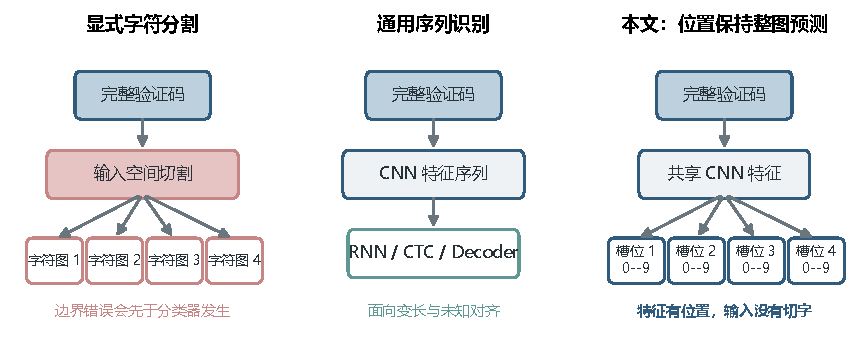
\includegraphics[width=\textwidth]{fig1_paradigms.pdf}
  \caption{三类识别路线的差别。显式分割先在输入空间产生字符子图；通用序列模型处理可变长和未知对齐；本文始终输入完整验证码，只在共享卷积特征上建立四个横向槽位。}
  \label{fig:paradigms}
\end{figure}

\begin{table}[htbp]
  \centering
  \caption{几类验证码或文本识别范式的比较}
  \label{tab:paradigm}
  \begin{tabularx}{\textwidth}{@{}lccccX@{}}
    \toprule
    方法 & 输入 & 显式切字 & 输出 & 变长支持 & 主要特点 \\
    \midrule
    分割后分类 & 整图到字符图 & 是 & 单字符类别 & 依实现而定 & 流程直观，但受分割上限约束 \\
    全局多输出 CNN & 整图 & 否 & 固定 $L\times C$ & 否 & 结构简单，适合长度固定任务 \\
    CRNN/CTC & 整图 & 否 & 字符序列 & 是 & 对齐灵活，模型与部署更复杂 \\
    本文 Position-DS & 整图 & 否 & $4\times10$ & 否 & 在特征空间保留四个横向位置 \\
    \bottomrule
  \end{tabularx}
\end{table}

\section{问题定义与数据集}

\subsection{任务定义}

输入为完整灰度验证码
\begin{equation}
  x\in[0,1]^{1\times32\times96},
\end{equation}
标签为 $y=(y_1,y_2,y_3,y_4)$，其中 $y_i\in\{0,\ldots,9\}$。模型一次前向传播输出
\begin{equation}
  f_\theta(x)\in\mathbb{R}^{4\times10}.
\end{equation}
四个位置的预测由同一幅完整图像共同产生。池化后形成的四个 feature slots 属于学习后的特征槽位，与输入图像的硬切片具有不同含义。

\subsection{数据采集与人工标注}

仓库公开数据共 3,203 张 PNG 图像，来自新优酷、次元城动画和饭团动漫三个实际来源。图\ref{fig:dataset}给出了未做亮度或对比度调整的样本。三类图像乍看相似，字体粗细、旋转方式和灰度仍有可见差别。这也是我们后来不再只看单一来源随机划分的原因。

三个正式采集批次各包含 1,000 张图片，另有 203 张早期预检样本。所有图像均保留采集时的 $128\times40$ 原始字节，并由人工逐张确认四位数字标签。模型预测不会自动回写为人工标签。

\begin{table}[htbp]
  \centering
  \caption{开放数据集的来源组成}
  \label{tab:dataset}
  \begin{tabular}{lrrr}
    \toprule
    来源 & 正式采集 & 预检样本 & 合计 \\
    \midrule
    次元城动画 & 1,000 & 1 & 1,001 \\
    饭团动漫 & 1,000 & 101 & 1,101 \\
    新优酷 & 1,000 & 101 & 1,101 \\
    \midrule
    合计 & 3,000 & 203 & 3,203 \\
    \bottomrule
  \end{tabular}
\end{table}

\begin{figure}[htbp]
  \centering
  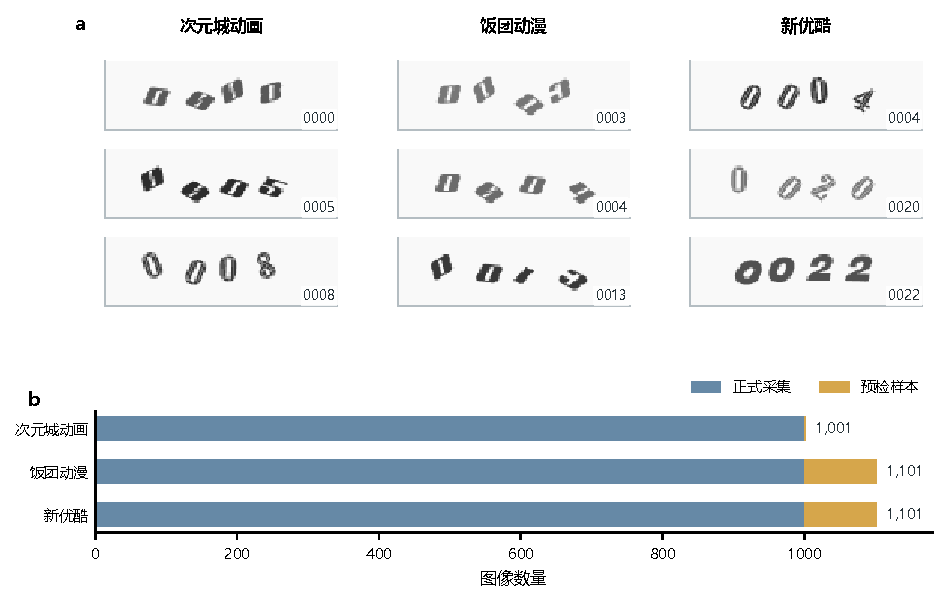
\includegraphics[width=\textwidth]{fig2_dataset.pdf}
  \caption{数据样例与来源构成。\textbf{a}，三个来源各展示三张正式采集样本，右下角为人工标签；图像仅按原始灰度显示。\textbf{b}，正式采集与预检样本数量。预检样本在元数据中单独标记，没有混写为正式批次。}
  \label{fig:dataset}
\end{figure}

数据 manifest 记录标签、来源、批次、用途、原始尺寸、样本 ID、相对路径与 SHA-256。保留这些字段直接服务于数据泄漏检查：当同一批次图像具有相似背景或生成参数时，批次信息能够帮助识别潜在的划分污染。

\subsection{预处理与受控增强}

推理预处理是确定性的：先将原图转为灰度图，再以最近邻插值缩放到 $96\times32$，最后除以 255 得到 float32 的 $[0,1]$ 数值。项目不使用 ImageNet 均值方差归一化，因而 Python 与端侧实现只需复现少量操作。

训练增强刻意保持在较弱范围：水平平移不超过 2 像素、垂直平移不超过 1 像素、旋转不超过 $2^\circ$、缩放范围为 $0.95$--$1.05$，并使用小幅亮度、对比度、低概率高斯模糊和标准差不超过 0.03 的高斯噪声。没有采用翻转、大角度旋转、随机裁剪、MixUp 或 CutMix。我们在这里的判断是，增强强度需要受到任务结构约束；对于 $1/7$、$2/3$、$6/8$ 等本来就容易混淆的数字，强形变可能改变与标签相关的笔画结构。

\subsection{数据划分与评估协议}

项目的评估协议随着对任务认识的深入逐步收紧，第一次实验时尚未完全固定。早期 746 张样本消融使用五折交叉验证，但缺少可用的批次隔离；随后增加 250 张单来源时间尾部留出和 184 张新优酷跨批次留出。最终阶段从三来源建立 481 张来源均衡留出集，其余样本分为 2,447 张训练集和 275 张验证集。

最终留出集中有 218 张图像曾出现在早期实验 manifest 中。它们没有进入最终模型的训练集，但架构选择已经间接接触过这部分数据。因此，本文统一使用“多来源留出评估”这一表述，并避免使用“完全未知的独立盲测”。这一限制不会让现有结果失去意义，但会缩小它能够支持的结论范围。

\section{整体识别系统与模型设计}

\subsection{从完整图像到四位预测}

图\ref{fig:pipeline}展示了系统的数据流。整张图里没有“切出四张字符图”这一步。四个输出来自共享卷积特征，只在最后分别读取横向槽位并进入独立分类头。

\begin{figure}[htbp]
  \centering
  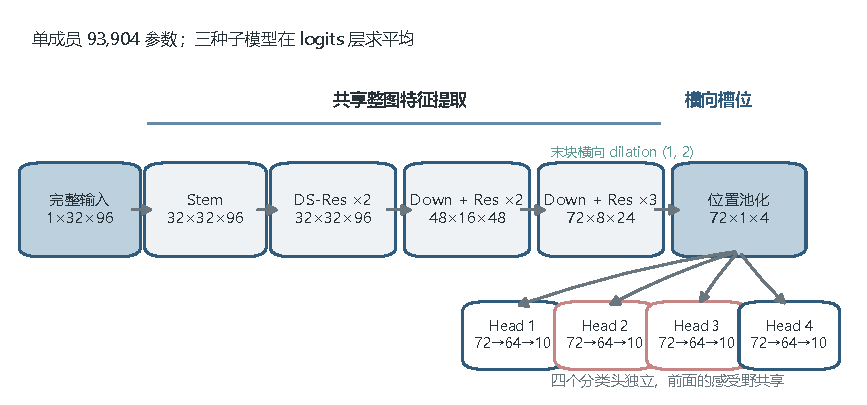
\includegraphics[width=\textwidth]{fig3_architecture.pdf}
  \caption{Position-DS 单成员结构。DS-Res 表示深度可分离残差块；末个残差块使用横向 dilation $(1,2)$。位置池化将共享特征压缩为四个槽位，再由四个独立分类头输出十类 logits。}
  \label{fig:pipeline}
\end{figure}

\subsection{全局展平模型与位置保持模型}

最初的 FlattenCaptchaCNN 使用三层 stride-2 卷积提取特征，将整个 feature map 展平后经一个线性层输出 40 个 logits。MediumCaptchaCNN 增加了通道数、池化和隐藏层，但仍然依赖全局联合表示。两者都属于整图预测；主要缺陷在于网络缺少从横向位置到输出位次的直接结构提示。

PositionCaptchaCNN 和 WidePositionCaptchaCNN 使用自适应平均池化，目标尺寸为 $(4,4)$。池化结果在宽度方向形成四个槽位，每个槽位保留跨高度的聚合特征，再由共享分类器预测一个数字。换言之，设计变化是
\begin{equation}
  \text{global flattened representation}
  \quad\longrightarrow\quad
  \text{global position-aware representation},
\end{equation}
这一变化仍然保持整图识别范式。

\subsection{Position-DS 网络}

最终 Position-DS 在保持位置建模的基础上重新设计了骨干网络。单成员的主要结构如下：

\begin{enumerate}
  \item $3\times3$ 卷积将单通道输入映射到 32 通道，接 Batch Normalization 和 SiLU 激活\cite{ioffe2015batchnorm,elfwing2018silu}；
  \item 32 通道阶段包含两个深度可分离残差块；
  \item 两次 stride-2 下采样依次扩展到 48 和 72 通道；
  \item 48 通道阶段包含两个残差块，72 通道阶段包含三个残差块，最后一块采用横向 dilation $(1,2)$；
  \item 自适应平均池化到 $(1,4)$，每个位置得到 72 维特征；
  \item 四个独立的 $72\rightarrow64\rightarrow10$ 分类头输出 $[B,4,10]$。
\end{enumerate}

深度可分离卷积将空间卷积与通道混合拆开，常用于降低移动端视觉模型的计算与参数开销\cite{howard2017mobilenets}。本模型的每个成员含 93,904 个可训练参数。四个独立分类头允许不同位置形成略有差异的判别边界，但它们仍共享前面的完整图像特征。

\subsection{三模型 logits 集成}

最终系统训练三个随机种子为 42、3407 和 20260716 的同构模型，并对 logits 求算术平均：
\begin{equation}
  \bar z=\frac{1}{3}\sum_{m=1}^{3}z^{(m)}.
\end{equation}
集成共有 281,712 个可训练参数。集成操作直接平均未经过 softmax 的 logits，从而保留每个类别的相对证据；各模型的 argmax 结果不参与平均。

\section{训练方法与评估指标}

\subsection{损失函数与优化}

四个位置分别计算交叉熵。最终训练使用位置权重 $(1.0,1.15,1.15,1.0)$ 和 0.02 的 label smoothing：
\begin{equation}
  \mathcal{L}=\frac{\sum_{i=1}^{4}w_i\,\mathcal{L}_{\mathrm{CE}}(z_i,y_i)}{\sum_{i=1}^{4}w_i}.
\end{equation}
中间两个位置在早期错误分析中更值得关注，因此获得稍高权重。优化器为 AdamW\cite{loshchilov2019adamw}。学习率从 $1.5\times10^{-3}$ 经 500 次 warmup 后按余弦退火至 $10^{-5}$。权重衰减为 $10^{-4}$，批大小为 32，梯度裁剪阈值为 1.0。

训练维护衰减率 0.999 的参数指数滑动平均。17,500 次更新后启用困难样本重放，将困难样本的抽样权重设为 2.0。在线困难样本挖掘的核心思想是把后期训练资源更多投入尚未学会的样本\cite{shrivastava2016ohem}；本文实现较为克制，只调整抽样权重，没有改变样本标签或自动生成新数据。

\subsection{指标与置信度}

设 batch 中共有 $B$ 张图片，每张四位。字符准确率和整码准确率分别为
\begin{align}
  \mathrm{CharAcc}
  &=\frac{1}{4B}\sum_{b=1}^{B}\sum_{i=1}^{4}
    \mathbb{I}(\hat y_{b,i}=y_{b,i}),\\
  \mathrm{ExactAcc}
  &=\frac{1}{B}\sum_{b=1}^{B}
    \mathbb{I}(\hat{\boldsymbol y}_{b}=\boldsymbol y_b).
\end{align}
汉明错误为每张图中预测错误的位置数均值：
\begin{equation}
  \mathrm{HammingError}
  =\frac{1}{B}\sum_{b=1}^{B}\sum_{i=1}^{4}
  \mathbb{I}(\hat y_{b,i}\ne y_{b,i}).
\end{equation}
对真实使用而言，一位错误就会使整个验证码失败，因此本文以 ExactAcc 为主要决策指标。推理置信度取四个位置最大类别概率的最小值：
\begin{equation}
  c(x)=\min_i\max_k\operatorname{softmax}(z_i)_k.
\end{equation}
这个定义会让最不确定的位置决定整码置信度，避免用平均值掩盖单个低置信字符。

\subsection{可复现训练与导出}

训练启动时冻结样本文件列表、split、超参数和随机状态；检查点保存模型、优化器、EMA、采样器和进度，续跑时重新校验上下文。评估训练完成后，先用留出集确定三个成员的更新数，再在全部 3,203 张冻结样本上重训生产模型，因此生产权重与评估权重相互独立。生产训练不生成用于宣传的训练集准确率，可信性能仍来自前述留出评估。

\section{实验演化与结果分析}

\subsection{从可学习性检查开始}

正式比较之前，我们先让模型在 32 张真实样本上过拟合到 100\% Train ExactAcc。这一结果只用于可学习性检查。它回答更早、更实际的问题：标签有没有读反，像素范围是否正确，损失能否反传，四个位置与标签能否对齐。若这些链路尚未确认，长训练只会把错误藏得更深。

\subsection{主要实验演化}

图\ref{fig:evolution}和表\ref{tab:evolution}汇总了仓库中可审计的实验阶段。图中的上升轨迹容易给人一种“模型按顺序公平竞赛”的印象，但各阶段的实验条件实际存在差异。背景色把四类评估协议分开；数据量、划分和训练预算也随阶段变化。这些结果适合回答项目怎样走到最终方案，不适合充当严格同条件排行榜。

\begin{figure}[htbp]
  \centering
  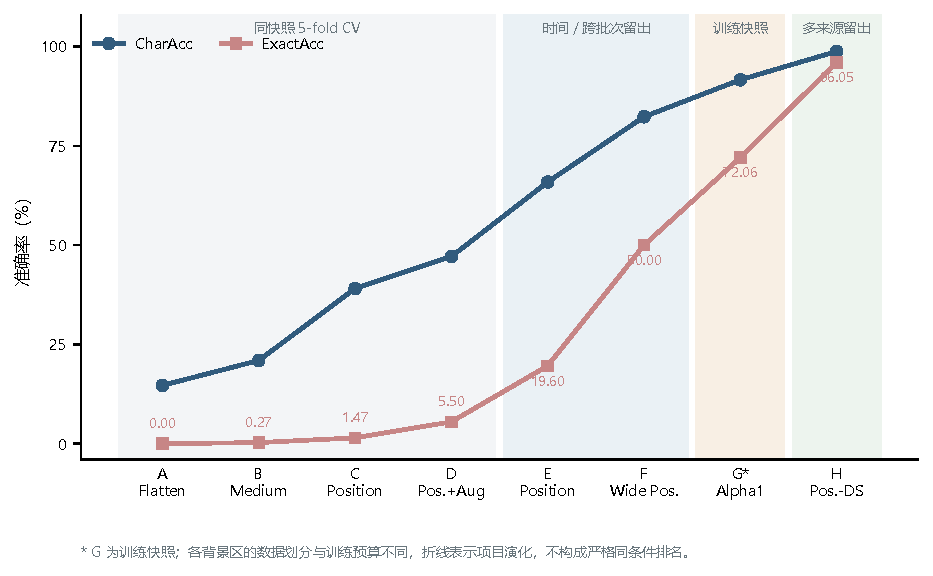
\includegraphics[width=\textwidth]{fig4_evolution.pdf}
  \caption{实验演化中的 CharAcc 与 ExactAcc 点估计。A--D 使用同快照五折交叉验证，E--F 为时间或跨批次留出，G 为训练快照，H 为多来源留出。不同背景区不可直接归因比较；连线仅帮助读者跟随项目演化。}
  \label{fig:evolution}
\end{figure}

\begin{table}[htbp]
  \centering
  \caption{模型与评估协议的实验演化}
  \label{tab:evolution}
  \resizebox{\textwidth}{!}{%
  \begin{tabular}{cllrrrr}
    \toprule
    阶段 & 模型 & 评估方式 & 训练数 & 评估数 & CharAcc & ExactAcc \\
    \midrule
    A & Flatten & 5-fold CV & 746 & 746 & 14.68\% & 0.00\% \\
    B & Medium & 5-fold CV & 746 & 746 & 20.96\% & 0.27\% \\
    C & Position & 5-fold CV，无增强 & 746 & 746 & 39.07\% & 1.47\% \\
    D & Position & 5-fold CV，轻量增强 & 746 & 746 & 47.15\% & 5.50\% \\
    E & Position & 时间留出 & 1,618 & 250 & 65.90\% & 19.60\% \\
    F & Wide Position & 新优酷跨批次留出 & 2,000 & 184 & 82.34\% & 50.00\% \\
    G & Wide Position 集成 & 训练快照 & 2,477 & 2,477 & 91.65\% & 72.06\%$^{*}$ \\
    H & Position-DS 集成 & 多来源留出 & 2,447 & 481 & 98.80\% & 96.05\% \\
    \bottomrule
  \end{tabular}}
  \vspace{0.4em}

  \raggedright\footnotesize $^{*}$训练快照指标，仅用于记录训练阶段表现，不作为独立泛化结果。
\end{table}

第一次结果并不好看。Flatten 的 ExactAcc 为 0\%。完整图像可以通过网络，展平表示却没有把四个位次组织起来。Medium 将 CharAcc 提高到 20.96\%，整码准确率仍只有 0.27\%。这次失败很重要：它迫使我们停止重复“再加一点容量”，转而检查模型究竟记住了什么空间关系。

Position 在同一批 746 张样本上的 CharAcc 提高到 39.07\%，加入轻量增强后达到 47.15\%。绝对性能仍然很低，却提供了方向性的证据：在不切割输入图像的前提下保留横向结构是有效的。随后，更多数据与更严格的留出方式让我们看到了泛化难度。4,218 参数 Position 在时间留出集上的 ExactAcc 为 19.60\%；扩大为 40,394 参数的 Wide Position 后，跨批次留出达到 50.00\%。到这一阶段，容量与位置先验都已成为实际瓶颈的一部分。

alpha1 三模型集成在 2,477 张训练快照上达到 72.06\% ExactAcc。这个数字一度看起来足够漂亮，但它只说明模型能拟合当时的数据。它不能与后续 481 张留出结果并列解释为泛化性能。我们仍把它写进正文，因为完整的实验史需要保留失败、过拟合与阶段性结果；学会对一个顺眼的数字保持距离，也是这次实践的一部分。

\subsection{最终多来源评估}

最终 Position-DS 三模型集成在 481 张留出图像中完整识别正确 462 张，1,924 个字符中错 23 个。总体与分来源结果见表\ref{tab:final}。三个来源的 ExactAcc 均达到 95\% 或以上，说明最终性能在三个来源上均保持较高水平。

\begin{table}[htbp]
  \centering
  \caption{Position-DS 三模型集成的多来源留出结果}
  \label{tab:final}
  \begin{tabular}{lrrrr}
    \toprule
    指标 & 总体（481） & 新优酷（161） & 次元城（160） & 饭团（160） \\
    \midrule
    CharAcc & 98.80\% & 98.45\% & 99.22\% & 98.75\% \\
    ExactAcc@1 & 96.05\% & 96.27\% & 96.88\% & 95.00\% \\
    HammingError & 0.0478 & 0.0621 & 0.0313 & 0.0500 \\
    \bottomrule
  \end{tabular}
\end{table}

\begin{figure}[htbp]
  \centering
  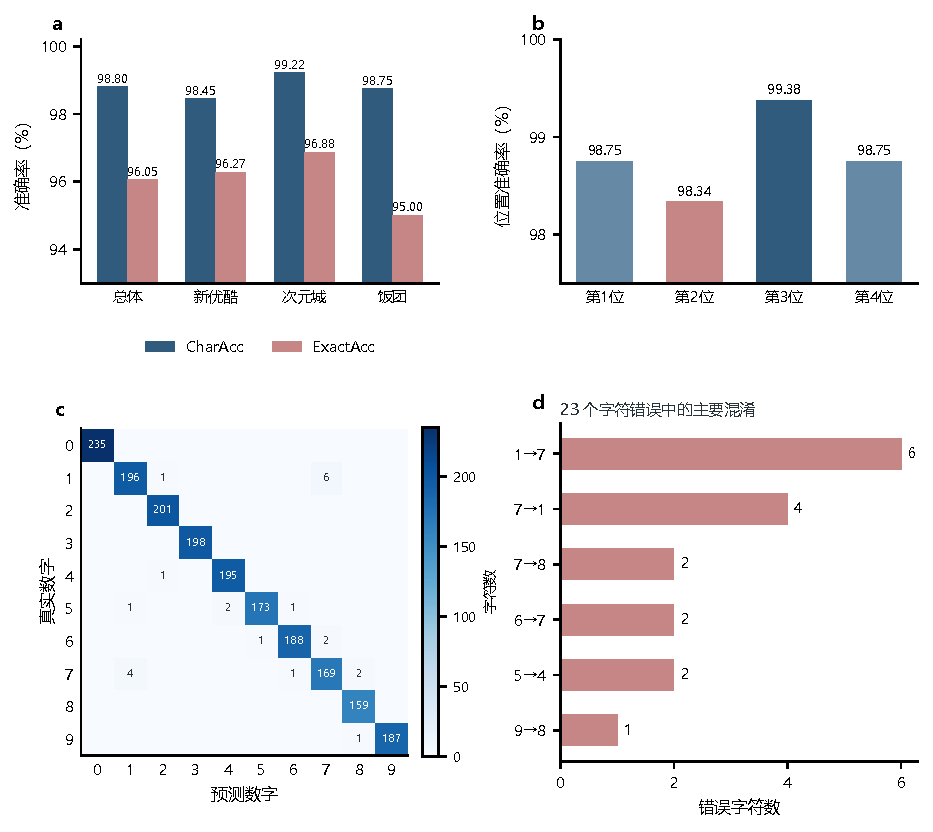
\includegraphics[width=\textwidth]{fig5_final_evaluation.pdf}
  \caption{最终多来源留出评估。\textbf{a}，总体及三个来源的字符准确率和整码准确率；\textbf{b}，四个位置的字符准确率；\textbf{c}，按真实数字与预测数字统计的混淆矩阵；\textbf{d}，非对角错误中出现次数最多的数字对。所有数值均来自同一 481 张留出集。}
  \label{fig:final-evaluation}
\end{figure}

总体 ExactAcc@2、@3 和 @5 分别为 98.34\%、98.54\% 和 98.75\%，说明多数错误样本的正确数字仍位于少量高概率候选中。四个位置准确率依次为 98.75\%、98.34\%、99.38\% 和 98.75\%，第二位略低但差距不大。从字符混淆矩阵看，错误主要集中在形态接近的 $1/7$ 等组合，在十个数字之间呈现明显的非均匀分布。

\subsection{实验告诉了我们什么}

如果只保留最后的 96.05\%，这组实验会显得过于顺利，也会掩盖最有价值的部分。表\ref{tab:lesson}把主要尝试、观察与后续决策重新放在一条线上。

\begin{table}[htbp]
  \centering
  \caption{失败、观察与设计决策}
  \label{tab:lesson}
  \begin{tabularx}{\textwidth}{@{}lXX@{}}
    \toprule
    尝试 & 观察 & 后续决策 \\
    \midrule
    Flatten global & 整码几乎不可识别 & 不切图，但要保留横向空间结构 \\
    Medium & 单纯增加全局头容量收益有限 & 优先改变归纳偏置 \\
    Position & 同批实验中明显改善 & 继续位置保持建模 \\
    Light augmentation & 泛化继续改善 & 保留不破坏笔画的弱增强 \\
    Temporal/cross-batch & 比同快照指标更困难 & 把来源和批次纳入评估设计 \\
    Wide Position & 跨批次 ExactAcc 达到 50\% & 扩充骨干但保持轻量 \\
    Position-DS + ensemble & 性能、体积与部署兼顾 & 冻结模型和导出契约 \\
    \bottomrule
  \end{tabularx}
\end{table}

不过，从 Wide Position 的 50.00\% 到最终 96.05\% 之间，同时改变了数据规模、划分、增强、训练日程、EMA、困难样本重放、位置权重、网络结构和集成方式。因此，现有实验不能严格推出“Position-DS 结构本身贡献了 46.05 个百分点”。本文更愿意把最终结果理解为一套共同设计的效果。

\section{工程实现与开源实践}

\subsection{ONNX 模型交付}

模型在 PyTorch 中训练\cite{paszke2019pytorch}，并导出为 ONNX opset 17。最终 \texttt{captcha.onnx} 将三个成员和 logits 平均封装为一个计算图，输入为 $[B,1,32,96]$，输出为 $[B,4,10]$。文件大小为 1,173,896 字节，约 1.12 MiB。

ONNX checker 已通过；在 8 张真实图像上，PyTorch 与 ONNX Runtime 输出的最大绝对 logits 误差为
\begin{equation}
  \max|z_{\mathrm{PyTorch}}-z_{\mathrm{ONNX}}|
  =1.5497208\times10^{-6},
\end{equation}
远低于项目约定的 $10^{-4}$。这里只比较 argmax 是不够的，因为两个实现可能碰巧预测相同类别，却在概率结构上已经明显偏离。logits 对齐把“模型可以打开”提高为更严格的数值契约。

\subsection{从研究仓库到实际软件}

模型的最初需求来自 Animeko 中真实媒体源的图片验证码流程。链路包括获取验证码、整图预处理、本地 ONNX 推理、自动提交，以及失败后的重试或人工回退。该功能通过 Animeko PR \#3172 合入下游项目\cite{animeko2026pr}。PR 记录同时保留了部署边界：Android 完成了实际测试，Desktop 与 iOS 当时只有实现与测试，尚未完成实机验证。这个事实不会抬高测试集准确率，却实实在在地改变了项目的质量要求。预处理必须跨平台复现，输入输出形状不能含糊，模型文件需要稳定哈希，低置信结果也要有退出路径。

仓库公开了训练代码、人工标注数据、实验结果、模型卡、数据卡、split、manifest、校验和与最小推理示例\cite{cnnforani2026repo}。
\subsection{责任边界}

验证码可能同时承担访问控制的一部分，因此模型的使用边界不能只由技术可行性决定。本项目限定于已获授权的兼容性研究、可复现实验和无障碍自动化，不应被用于绕过未授权服务的访问限制。三类来源名称仅用于科研溯源，也不表示来源站点认可本项目。

\section{讨论}

\subsection{位置建模与隐式切字的区别}

图\ref{fig:paradigms}中最容易混淆的是第一列和第三列。显式字符分割发生在输入空间：
\begin{equation}
  x\rightarrow(x_1,x_2,x_3,x_4)
  \rightarrow(y_1,y_2,y_3,y_4).
\end{equation}
本文方法发生在学习后的特征空间：
\begin{equation}
  x\rightarrow F_\theta(x)
  \rightarrow(f_1,f_2,f_3,f_4)
  \rightarrow(y_1,y_2,y_3,y_4).
\end{equation}
后者始终保留完整输入和共享感受野。$f_i$ 表示横向位置槽位，与从原图裁出的第 $i$ 个字符具有不同含义。强调这一区别可以准确说明先验加入的位置：字符边界没有被预先决定，位置信息则被有意保留下来。

\subsection{专用模型与通用序列模型的取舍}

CRNN、CTC 或 Transformer 能处理更复杂的长度和对齐关系，但本文任务并不需要 EOS、动态路径或自回归解码。固定四位输出使结构更小、推理接口更稳定，也更容易做跨语言数值对齐。代价同样明确：一旦验证码改为可变长度、加入字母或改变布局，当前四头模型不能直接适用。本文只支持一个较窄的结论：当任务约束真实存在且长期稳定时，利用这些约束可以换取更简单的系统。该实验不足以推出“专用 CNN 普遍优于序列模型”。

\subsection{尚未闭环的问题}

本课程项目仍留下几项值得继续完成、但不妨碍现阶段总结的问题：

\begin{itemize}
  \item 最终 481 张留出集中有 218 张参与过早期方案选择；一个全新的三来源 blind set 才能给出更干净的泛化估计。
  \item 当前缺少在同一 train/validation/test split、同一训练预算下对 Flatten、Position、Wide Position、Position-DS 的统一复跑，因此各结构的净贡献尚未完全分离。
  \item 没有与 MobileNet、CRNN/CTC 等替代模型做同预算 benchmark，不能回答专用位置模型相对通用轻量模型的精确优势。
  \item 数据只覆盖三个来源、四位纯数字和相近的图像生成分布，不能外推为通用 OCR 或任意验证码识别能力。
  \item Python/ONNX logits 已完成对齐；纯 Kotlin 前向若不依赖 ONNX Runtime，仍需在 Animeko 工程内完成同一输入下小于 $10^{-4}$ 的 40 logits 对齐。
\end{itemize}

这些缺口也给出了自然的后续工作次序：先补全新盲测，再做统一预算消融，最后才有必要扩大模型族比较。对于一篇结课论文而言，诚实保留这条未完成路径，比把不同阶段的数字强行拼成一个闭环结论更可靠。

\section{结论}

本文围绕固定四位数字验证码完成了一次从任务建模、实验试错到模型交付的复盘。模型始终以完整验证码为输入，并在一次前向传播中输出四个位置的十分类结果；位置池化在特征空间提供横向归纳偏置，输入空间始终保持完整验证码。早期实验表明，简单展平全局特征和单纯增加容量都不足以解决问题，位置保持结构与受控增强带来了明确改善。随着数据规模、骨干网络和训练策略继续完善，最终 Position-DS 三模型集成在 481 张多来源留出集上达到 96.05\% ExactAcc，并形成约 1.12 MiB 的可部署 ONNX 模型。

我们更愿意把项目的价值理解为一种方法选择：面对高度约束的实际问题，先承认任务先验，再选择足够而不过度复杂的模型；面对失败实验，优先检查表示与任务的匹配程度，再决定是否增加网络容量；面对一个漂亮数字，则继续追问它来自何种数据划分、是否经历方案选择、能否在另一种运行时复现。Position-DS 是这段过程的最终实现，但真正贯穿本文的，是从完整图像到位置化整图预测的认识变化。

\clearpage
\addcontentsline{toc}{section}{参考文献}
\begin{thebibliography}{99}

\bibitem{vonahn2003captcha}
L. von Ahn, M. Blum, N. J. Hopper, and J. Langford.
\newblock CAPTCHA: Using Hard AI Problems for Security.
\newblock In \emph{Advances in Cryptology -- EUROCRYPT 2003}, pp. 294--311, Springer, 2003.
\newblock doi: \href{https://doi.org/10.1007/3-540-39200-9_18}{10.1007/3-540-39200-9\_18}.

\bibitem{chen2017survey}
J. Chen, X. Luo, Y. Guo, Y. Zhang, and D. Gong.
\newblock A Survey on Breaking Technique of Text-Based CAPTCHA.
\newblock \emph{Security and Communication Networks}, 2017:1--15, 2017.
\newblock doi: \href{https://doi.org/10.1155/2017/6898617}{10.1155/2017/6898617}.

\bibitem{goodfellow2014multidigit}
I. J. Goodfellow, Y. Bulatov, J. Ibarz, S. Arnoud, and V. Shet.
\newblock Multi-digit Number Recognition from Street View Imagery using Deep Convolutional Neural Networks.
\newblock In \emph{International Conference on Learning Representations}, 2014.
\newblock \url{https://arxiv.org/abs/1312.6082}.

\bibitem{graves2006ctc}
A. Graves, S. Fern\'andez, F. Gomez, and J. Schmidhuber.
\newblock Connectionist Temporal Classification: Labelling Unsegmented Sequence Data with Recurrent Neural Networks.
\newblock In \emph{Proceedings of the 23rd International Conference on Machine Learning}, pp. 369--376, 2006.
\newblock doi: \href{https://doi.org/10.1145/1143844.1143891}{10.1145/1143844.1143891}.

\bibitem{shi2017crnn}
B. Shi, X. Bai, and C. Yao.
\newblock An End-to-End Trainable Neural Network for Image-Based Sequence Recognition and Its Application to Scene Text Recognition.
\newblock \emph{IEEE Transactions on Pattern Analysis and Machine Intelligence}, 39(11):2298--2304, 2017.
\newblock doi: \href{https://doi.org/10.1109/TPAMI.2016.2646371}{10.1109/TPAMI.2016.2646371}.

\bibitem{thobhani2020captcha}
A. Thobhani, M. Gao, A. Hawbani, S. T. M. Ali, and A. Abdussalam.
\newblock CAPTCHA Recognition Using Deep Learning with Attached Binary Images.
\newblock \emph{Electronics}, 9(9):1522, 2020.
\newblock doi: \href{https://doi.org/10.3390/electronics9091522}{10.3390/electronics9091522}.

\bibitem{ma2020neuralcaptcha}
Y. Ma, G. Zhong, W. Liu, J. Sun, and K. Huang.
\newblock Neural CAPTCHA Networks.
\newblock \emph{Applied Soft Computing}, 97:106769, 2020.
\newblock doi: \href{https://doi.org/10.1016/j.asoc.2020.106769}{10.1016/j.asoc.2020.106769}.

\bibitem{ioffe2015batchnorm}
S. Ioffe and C. Szegedy.
\newblock Batch Normalization: Accelerating Deep Network Training by Reducing Internal Covariate Shift.
\newblock In \emph{Proceedings of the 32nd International Conference on Machine Learning}, pp. 448--456, 2015.

\bibitem{elfwing2018silu}
S. Elfwing, E. Uchibe, and K. Doya.
\newblock Sigmoid-Weighted Linear Units for Neural Network Function Approximation in Reinforcement Learning.
\newblock \emph{Neural Networks}, 107:3--11, 2018.
\newblock doi: \href{https://doi.org/10.1016/j.neunet.2017.12.012}{10.1016/j.neunet.2017.12.012}.

\bibitem{howard2017mobilenets}
A. G. Howard, M. Zhu, B. Chen, et al.
\newblock MobileNets: Efficient Convolutional Neural Networks for Mobile Vision Applications.
\newblock \emph{arXiv preprint arXiv:1704.04861}, 2017.
\newblock \url{https://arxiv.org/abs/1704.04861}.

\bibitem{loshchilov2019adamw}
I. Loshchilov and F. Hutter.
\newblock Decoupled Weight Decay Regularization.
\newblock In \emph{International Conference on Learning Representations}, 2019.
\newblock \url{https://openreview.net/forum?id=Bkg6RiCqY7}.

\bibitem{shrivastava2016ohem}
A. Shrivastava, A. Gupta, and R. Girshick.
\newblock Training Region-Based Object Detectors with Online Hard Example Mining.
\newblock In \emph{Proceedings of the IEEE Conference on Computer Vision and Pattern Recognition}, pp. 761--769, 2016.
\newblock doi: \href{https://doi.org/10.1109/CVPR.2016.89}{10.1109/CVPR.2016.89}.

\bibitem{paszke2019pytorch}
A. Paszke, S. Gross, F. Massa, et al.
\newblock PyTorch: An Imperative Style, High-Performance Deep Learning Library.
\newblock \emph{Advances in Neural Information Processing Systems}, 32:8024--8035, 2019.

\bibitem{animeko2026pr}
proffitteoy.
\newblock feat(media-source): 添加多平台图片验证码自动处理.
\newblock GitHub pull request \#3172, 2026. Merged 2026-07-24; accessed 2026-09-07.
\newblock \url{https://github.com/open-ani/animeko/pull/3172}.

\bibitem{cnnforani2026repo}
proffitteoy.
\newblock CNN for Ani: A Reproducible Four-Digit CAPTCHA CNN Research Repository.
\newblock Version 1.0.0, GitHub repository, 2026. Released 2026-07-17; accessed 2026-09-07.
\newblock \url{https://github.com/proffitteoy/CNN-for-Ani}.

\end{thebibliography}

\end{document}
